\chapter{Processo}
Foi definido um processo de Engenharia de Requisitos ágil, fundamentado no SAFe 4.0, porém sem a utilização do nível de de fluxo de valor. Pois foi observado que ele não era necessário no nosso contexto, e que não agregaria nenhum valor real, uma vez que se trata de um projeto pequeno para uma empresa júnior da Universidade de Brasília.

\begin{description}
\item[Especialista do Negócio] É o \textit{stakeholder} que detém o conhecimento do negócio, do contexto organizacional e da visão do produto.    
\item[Product Owner (P.O.)] É o membro do time que fica responsável pela definição das histórias e pela priorização do \textit{Team Backlog}, além de participar do planejamento e validação da \textit{sprint} definindo os seus objetivos.
\item[Product Manager (P.M.)] De acordo com Leffingwell~(\citeyear{leffingwell}), cabe ao P.M.: manter a visão e o \textit{Program Backlog}, priorizar \textit{features}, manter o \textit{Roadmap}, gerenciar o conteúdo da \textit{Release} e manter e priorizar o \textit{Porfolio Backlog}. As atividades realizadas pelo P.M. acontecem nos níveis Portfolio e Programa.
\item[Scrum Master] Seu papel é dar assistência para o resto da equipe a fim de extrair a máxima perfomance, ele é de certa forma o líder do time~\cite{leffingwell}.
\item[Time] É composto por toda a equipe, desenvolvedores, \textit{designers} e etc.
\end{description}

\section{Big picture do processo}
  \begin{figure}[!htbp]
    \centering
    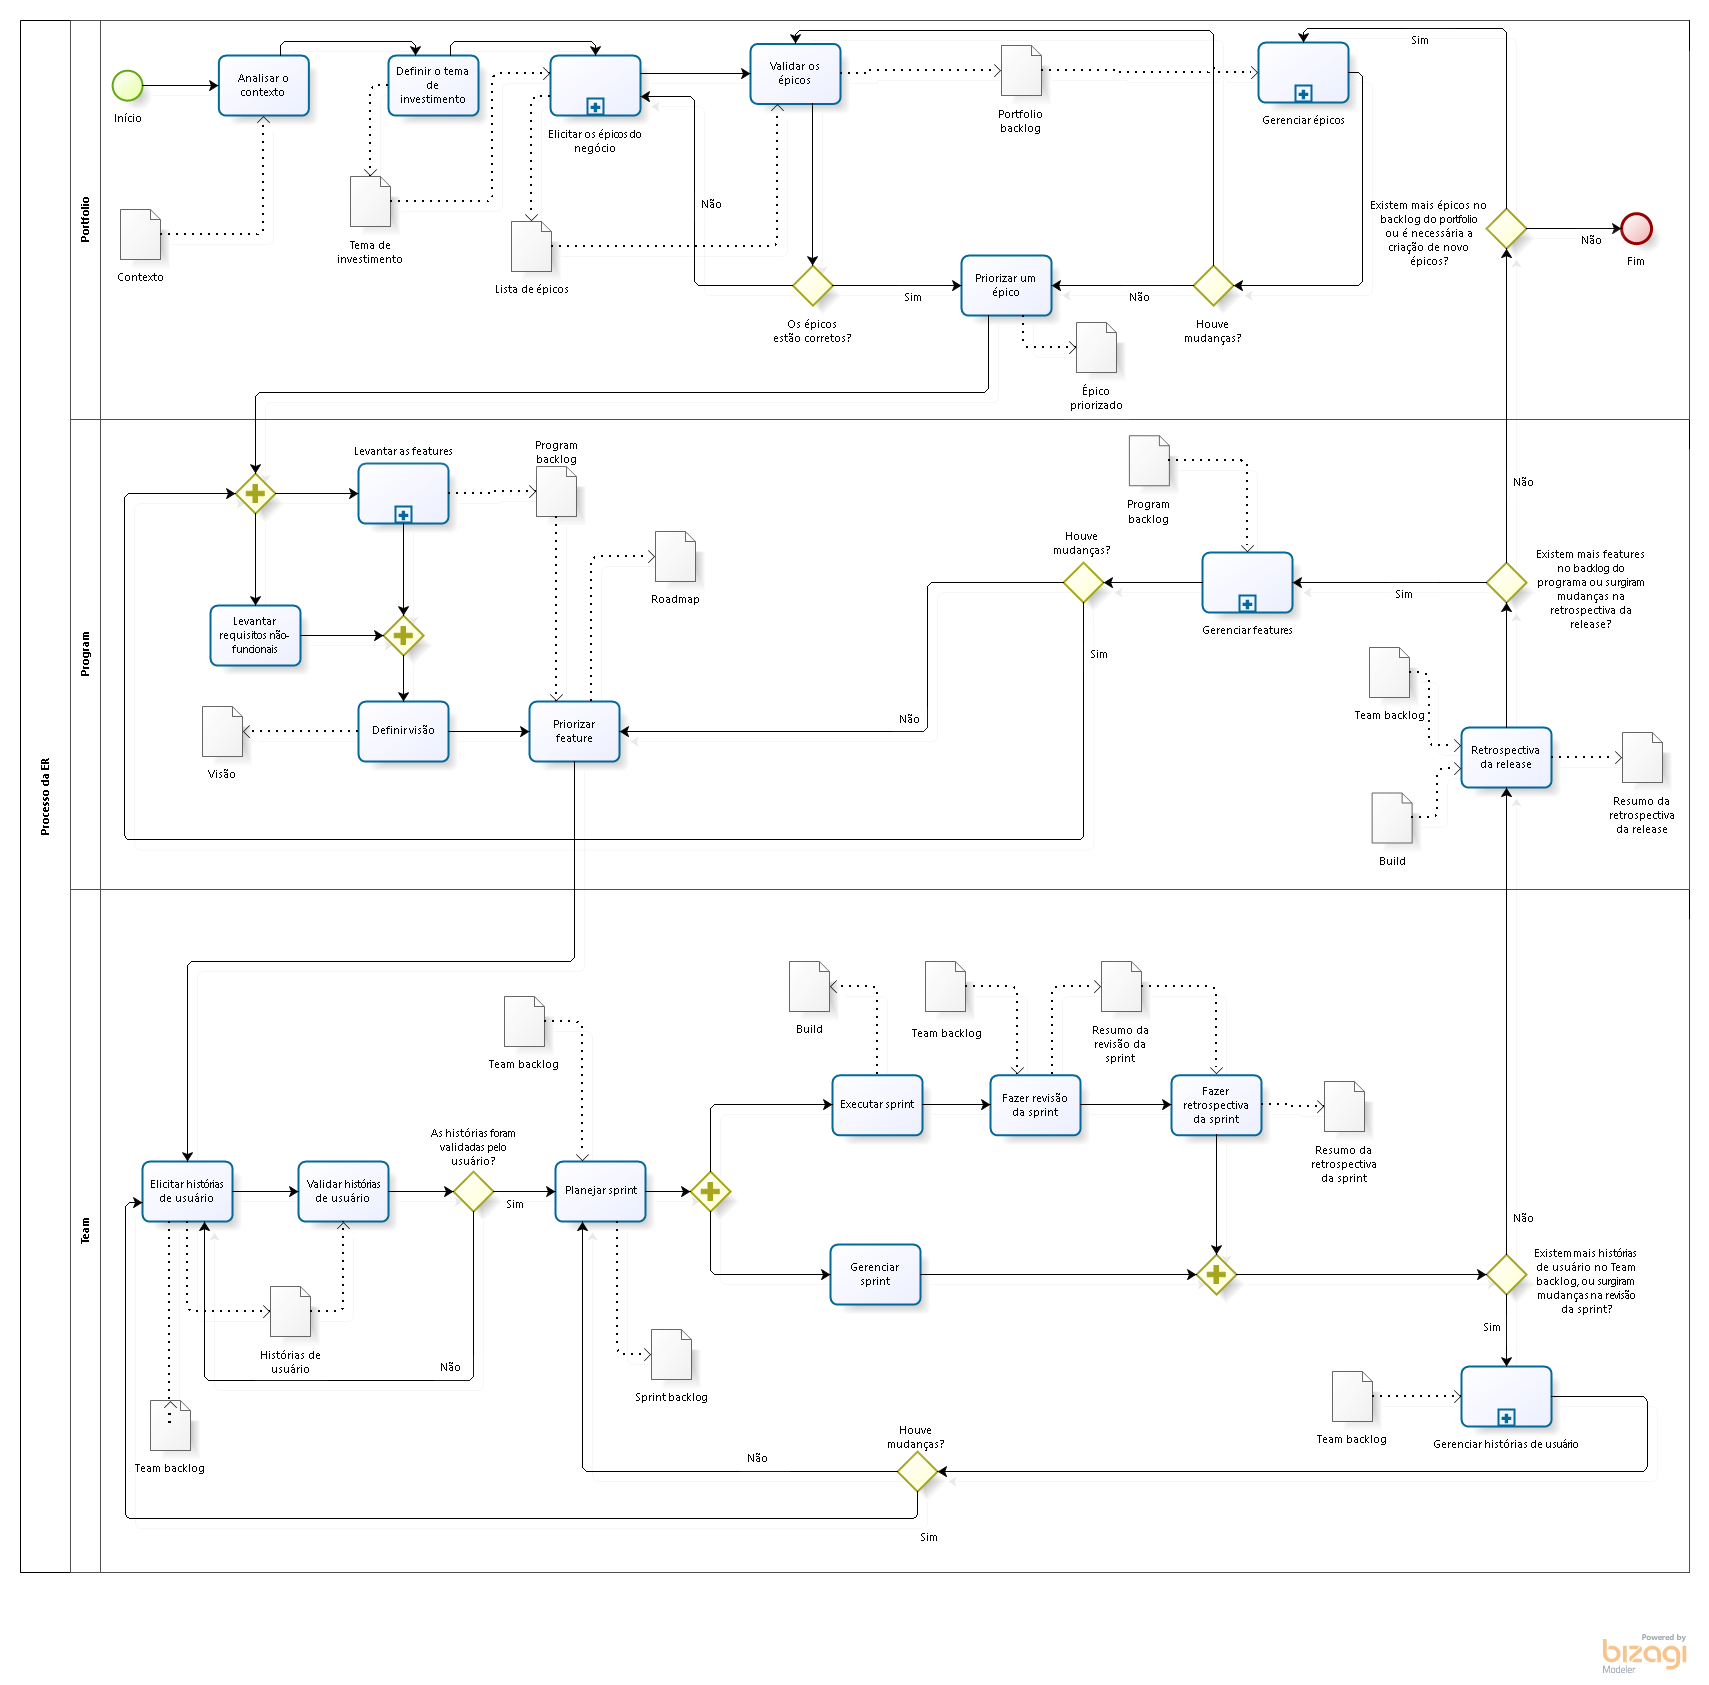
\includegraphics[scale=0.3]{figuras/Processo_v1-2}
    \caption[Big picture do processo.]{Big picture do processo. \footnotemark}
    \label{processo}
  \end{figure}